%\subsection{Portfolio f\"ur Input Data und Replication Package (Gr\"o\ss{}e entspricht der Anzahl)}
%\begin{figure}
\begin{center}
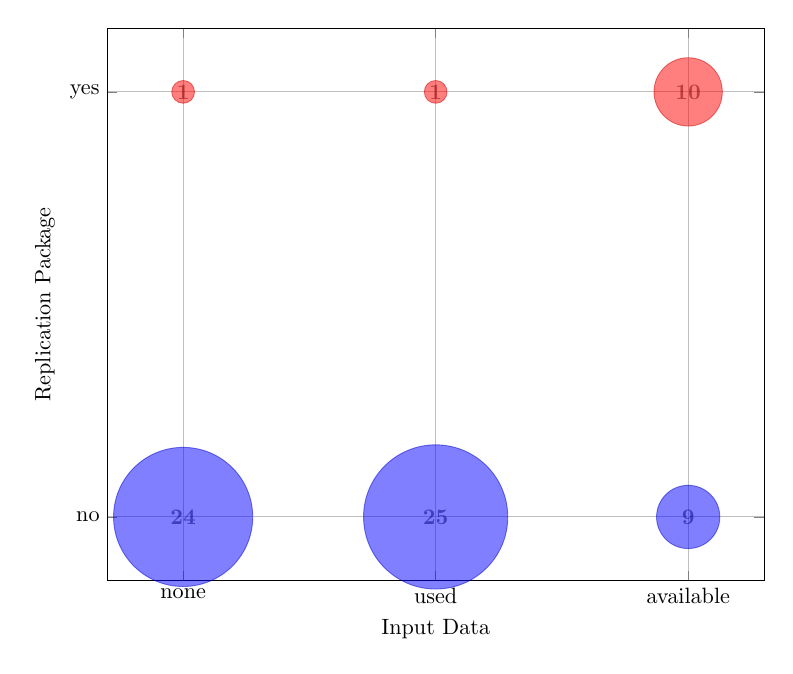
\begin{tikzpicture}[scale=.8]
\begin{axis}[scatter,
    width=.99\linewidth,
    cycle multi list=Spectral,
    every axis plot/.append style={draw, fill, fill opacity=0.5},
    scatter src=y,
    nodes near coords style={color=black,font=\small},
    enlargelimits=0.15,
    %x tick label style={rotate=45,anchor=east},
    xtick={0,1,2}, xticklabels={none,used,available},
    xlabel={Input Data},
    ytick={0,1}, yticklabels={no,yes},
    ylabel={Replication Package},
    grid=both
]

\addplot[mark size=31.429,opacity=0.5,text=black] coordinates { (0,0) } node[text=black,font=\bfseries] {24};
\addplot[mark size=5.143,opacity=0.5,text=black] coordinates { (0,1) } node[text=black,font=\bfseries] {1};
\addplot[mark size=32.571,opacity=0.5,text=black] coordinates { (1,0) } node[text=black,font=\bfseries] {25};
\addplot[mark size=5.143,opacity=0.5,text=black] coordinates { (1,1) } node[text=black,font=\bfseries] {1};
\addplot[mark size=14.286,opacity=0.5,text=black] coordinates { (2,0) } node[text=black,font=\bfseries] {9};
\addplot[mark size=15.429,opacity=0.5,text=black] coordinates { (2,1) } node[text=black,font=\bfseries] {10};


\end{axis}
\end{tikzpicture}
\end{center}
%\caption{Portfolio f\"ur Input Data und Replication Package (Gr\"o\ss{}e entspricht der Anzahl)}\label{fig:port_inputdata_replicationpackage}
%\end{figure}

